%	Copyright (C) 2013 Systems Engineering Group
%
%	CHANGELOG:
%       2005-10-10 - corrected and extended. 
%       2013-01-28 - adjusted sections and explanation
%		2020-11-18 - basic content of hand-in


\documentclass[a4paper,10pt,twoside]{article}
\pagestyle{headings}
\usepackage{a4wide}
\usepackage{graphicx}
\usepackage[utf8]{inputenc}
\usepackage[spanish]{babel}
\usepackage{csquotes}
\graphicspath{ {./images/} }
\usepackage[colorlinks,hyperfigures,backref,bookmarks,draft=false]{hyperref}

\title{Disaggregated Compute and Storage for Distributed LSM-based Databases}
\author{Zidi Chen}
\date{\today}

\begin{document}

\maketitle

\begin{abstract}
Here you provide a very short intoduction into your topic and sum up your hand-in. 
It is important to highlight the main issues to be discussed in your hand-in here.
\end{abstract}

\tableofcontents

\section{Introduction of the Research Field}

Distributed databases like MongoDB, TiDB have been more widely used in many large-scale services senarios.
But in many cases, distributed databases could suffer performace degradation and low utilizationn from skew, backgroud operatio and compaction.
The paper~\textit{Hailstorm: Disaggregated Compute and Storage for Distributed LSM-based Databases} \cite{mainpaper}introduces Hailstorm, a system that disaggregates storage and compute for distributed LSM-based databases.
It shows that Hailstorm achieves load balance in many MongoDB deployments with skewed workloads, improving the average throughput by 60$\%$, while decreasing tail latency by as much as 5×.


\section{Basics}

\subsection{LSM-Tree}

Traditional disk-based index structures such as the B-tree will effectively double the I/O cost of the transaction to maintain an index such as this in real time, increasing the total system cost up to fifty percent. 
Hence Log-structured merge tree (LSM-Tree) has been widely used by many distributed databases, as it provides efficient indexing for a key-value store with a high rate of inserts and deletes.
The LSM-tree uses an algorithm that defers and batches index changes, cascading the changes from a memory-based component through one or more disk components in an efficient manner reminiscent of merge sort. 
During this process all index values are continuously accessible to retrievals (aside from very short locking periods), either through the memory component or one of the disk components.

\subsection{Compaction in LSM KV Stores}

Compaction is a very critical mechanism in a system based on LSM-Tree. 
Log append method brings high-throughput writes. 
As the sstable continues to be written, more and more files will be opened by the system, and the accumulated data changes (updates, deletes) operations for the same key will increase. 
Since sstable is immutable, the data in the memory will reaches the upper limit in certain layer.
In order to reduce the number of files and clean up invalid data in time, the compaction mechanism was introduced to optimize read performance and space.
\newline
Compaction can be implemented in many ways. For example, RocksDB implements Tiered+Leveled, termed Level compaction.\cite{RocksDB_compaction_algo1}. 
\newline
Generally, in LSM tree, each level contains multiple partitions of data sorted by keys. When  compaction will be triggered by continuously recycling old version data and merging multiple layers into one layer through periodic background tasks.
The basic procedure goes as following:
\begin{figure}[h]
    \centering
	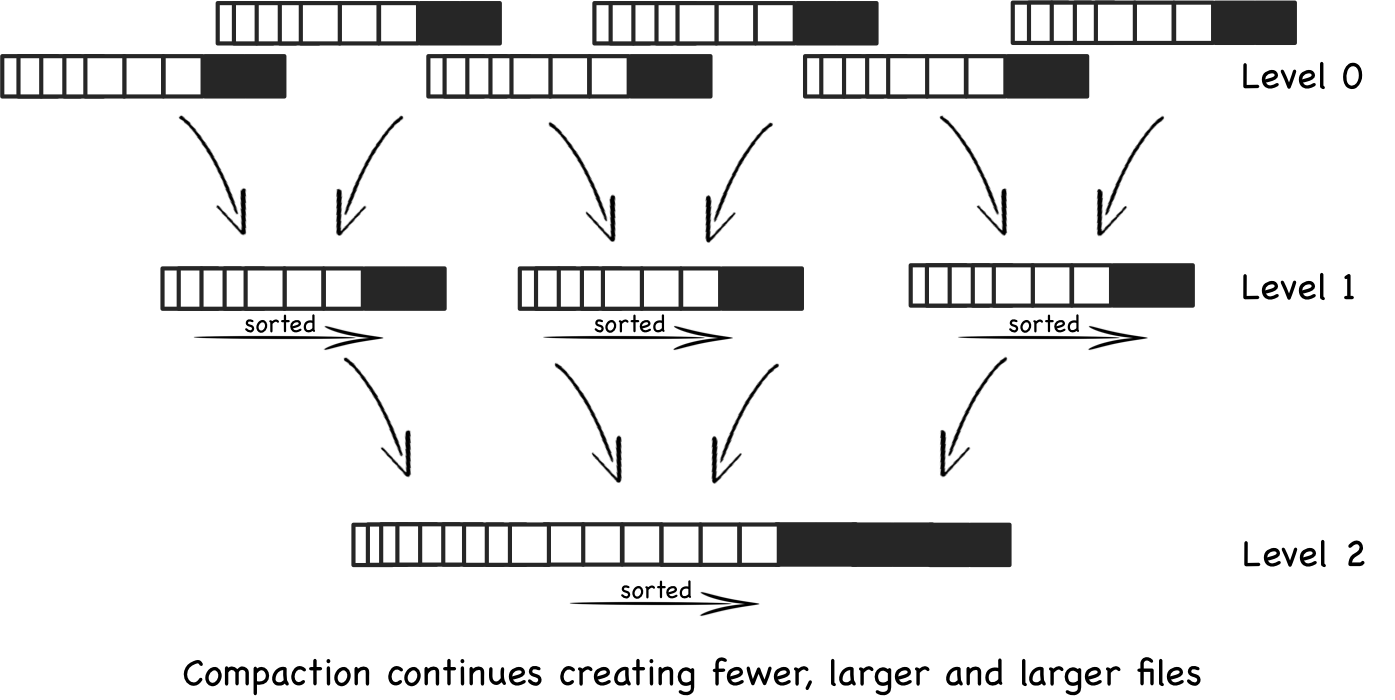
\includegraphics[scale=0.3]{LSM_Tree1.png}
    \caption{LSM Tree}
    \label{fig:mesh1}
\end{figure}
\newline
As is shown in Figure. Compaction into level N (L(n)) merges data from L(n-1) to L(n), where data is rewirted into the new level. 
In original paper of LSM tree, all data from L(n-1) is merged into L(n). 
In morden distributed databases such as LevelDB and RocksDB, overlapping data is eliminated, therefore for most time, only some data will be merged into new level.
\newline
Generally, LSM tree will continuously compact key-value pairs ,and the compaction and disk flushes will trigger big writes, which will cause significantly overheads due to I/O amplifications.


\subsection{Tow-level Sharding}
Sharding is widely used in distributed databases. Large data sets or high throughput applications can challenge the capacity of one single server.
Each area has the same schema and columns, but each table has completely different rows. 
Similarly, the data stored in each partition is unique and has nothing to do with the data stored in other partitions.
Sharding divides a piece of data into two or more smaller blocks, called logical shards.
Then, logical shards are distributed on separate database nodes, called physical shards.
Physical shards can hold multiple logical shards. 
Nevertheless, the data stored in all shards collectively represent the entire logical data set.
\newline
A tow-level sharding way is introduced in the paper\cite{mainpaper}. 
Hailstorm uses a tow-step data assignment scheme, where data objects are dynamically assigned to different partitions, 
so that the system could react better to the changes in the workfload and perform better load balance.
The target LSM-based databases still use the filesystem solution to redistribute data blocks into different nodes uniformly.


\subsection{Skew in Distributed Databases}

Distributed databases \cite{mongodb,tidb} are designed for large-scale data storage, which usually run on multiple nodes in the same,
or even partitioned networks.
Distributed database use sharding to tore larger dataset and handle additional requests by distributing the data among multiple machines.
The database engine translates user queries into individual queries that are routed to one or multiple database instances for execution.
Therefore, the database may suffer skew issue, where keys are unevenly to different nodes, which could cause uneven access and some nodes may become the hotsopt.
This could lead to globally performance degradation.



\section{Previous and Related Work}

\subsection{Skew in Distributed Databases}

Previously proposed solutions to eliminate skew in several ways.
MongoDB introduces a balancer to mitigate imbalanced shards\cite{MongoDB_balancing1}.
Some manual operations can also be performed, e.g., moving "hotspot" chunks manually to address the imbalances. 
In practice, some table related operations will also work, e.g., spliting one table into several sub-tables.


\subsection{Compaction and performance degradation}
Compaction may cause severe I/O performance degradation in LSM-based distributed databases, 
as it merges multiple tables and writes back to disk, which will typically comsue large I/O and CPU computing resources.
A benchmark test is conducted in the paper\cite{mainpaper}, 
\begin{displayquote}
	Profiling this particular experiment
	reveals that storage is saturated as I/O bandwidth remains
	almost constantly close to 320 MB/s, the maximum write
	bandwidth for our SSD. We also observe peaks of CPU utilization
	when compaction tasks run. 
\end{displayquote}
\begin{figure}[h]
    \centering
	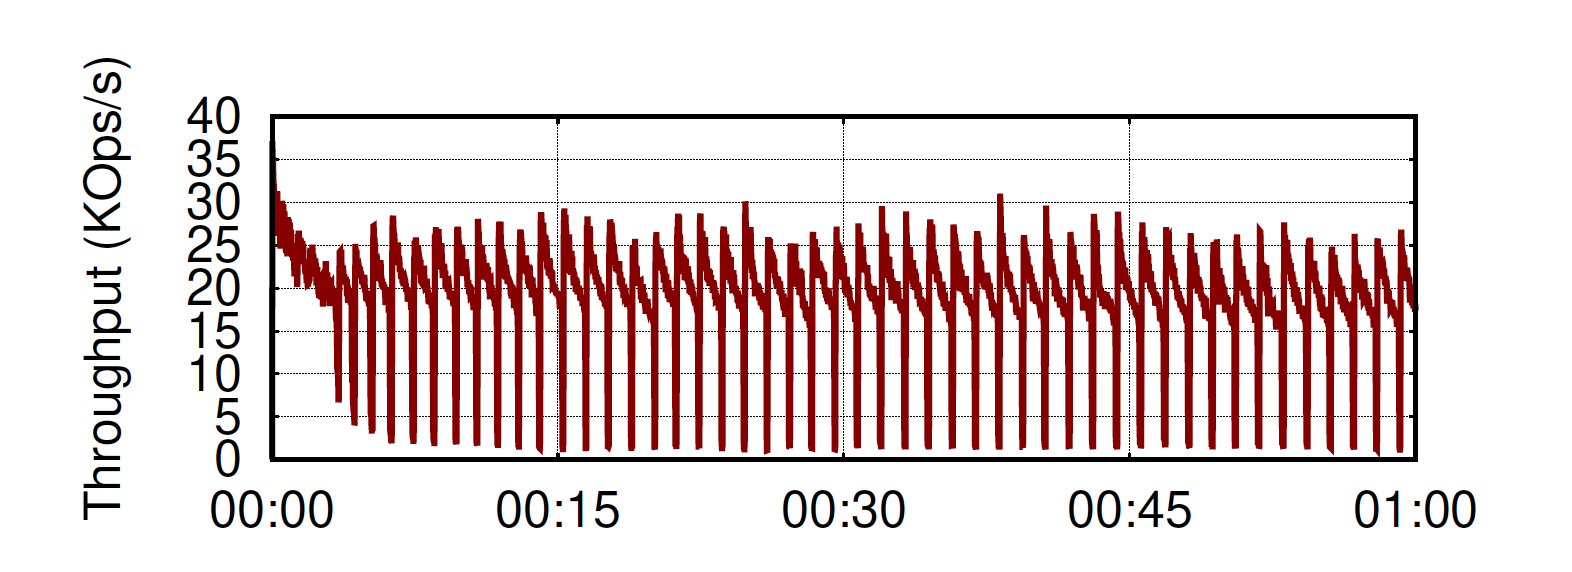
\includegraphics[scale=0.3]{Campaction perf.png}
    \caption{Embedded RocksDB throughput over time (HH:mm) on
	a node equipped with an Intel S3500 Series SSD using the YCSB
	A [38] workload (50$\%$ reads and 50$\%$ writes).}
    \label{fig:mesh1}
\end{figure}
Some solutions \cite{7569086} try to optimize the LSM-tree structure\cite{Yao2017ALC}, to introduce larger memory to cache more KV items, 
to leverage some specific characteristic of different devices \cite{10.1145/3033273, 10.5555/2813767.2813783}, or to reduce the number of the levels\cite{SMRDB}.
These solutions are mostly aimed at LSM-tree structure on individual nodes, but they don't take the utilization of other nodes in consideration.

\subsection{Distributed Databases with LSM Storage Engines}
TODO: sharding will not work

\subsection{Summary}
It can be shown from the previous work that skew will cause severe performance degradation, and the database system suffer from I/O brusts due to compaction and disk flushing.
Hailstrom tries to solve these problems by disaggregate resources to address load balancing at database and storage layers seperately.

\section{Hailstrom: disaggregate compute and storage}

\subsection{Design principles}


Describe the solution of the given paper, but do not copy it or repeat all of its details.
Present and explain the main concepts. 
%Do not forget to cite the paper~\cite{mainpaper} you have been assigned/chosen.
Note that you should rename this section. 

\section{Evaluation}

Present and discuss measurements, experiments, examples, ... but do not repeat the entire evaluation of the original paper.
\emph{Cite} all figures and tables copied form other papers.
You can keep this section short and focus on the aspects that were improved by the paper compared to existing approaches.

\section{Discussion}

What is bad about your paper? 
What are the good points? 
Mention criticism and ideas for improvement that you thought about while researching the topic.

\section{Conclusion}

Sum up your paper and the discussion points.

\bibliographystyle{unsrt}
\bibliography{handin} 

\end{document}
